\section{Adaptive Mesh Refinement (AMR)}
\subsection{Goals} %{{{
In this tutorial, we show how to use the mesher BAMG to run a simulation with AMR:
\begin{itemize}
	\item Learn how to set up the AMR properties and a refinement criterion;
	\item Run a transient simulation with AMR using the MISMIP3d setup to track the grounding line migration.
\end{itemize} 

Go to \verb@trunk/examples/AMR/@ to do this tutorial.
%}}}
\subsection{Introduction}
The \verb@runme.m@ file and \verb@mismip.par@ go through the steps and basic structure to set up and run the MISMIP3d experiment with adaptive mesh refinement to track the grounding line positions. The \verb@runme.m@ script is set up as three distinct steps, saving the model at each stage:
\begin{enumerate}
	\item Mesh generation
	\item Parameterization
	\item Transient solution with AMR
\end{enumerate}

\subsection{Mesh Generation}
Run step 1 in \verb@runme.m@ to generate an unstructured coarse mesh on a 800 x 50 km domain with typical element edge length of 10,000 m (10 km).  This coarse mesh shown here has 820 elements and 496 vertices. To plot your coarse mesh, use \verb@plotmodel(md,'data','mesh','fontsize',12);@:
\begin{figure}[H]
	\begin{center}
		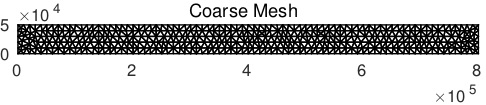
\includegraphics{/assets/img/tutorials/amr/amr_coarse_mesh.jpg}
	\end{center}
\end{figure}

\subsection{Parameterization}
Run step 2 in \verb@runme.m@ to define the model parameters. First we call on standard parameters defined in the \verb@mismip.par@ file (bed and ice geometry, sliding velocity, material properties, etc.). Then we define AMR-specific parameters to run an AMR transient simulation (resolution at the grounding line, distance to the grounding line used as criterion, ratio between two consecutive edges, etc.).

The MISMIP3d domain is initially set up as a 100 m thick slab of ice. The MISMIP3d bed is defined as $r=-100-x/1000$ (in [m], negative if below sea level). The surface mass balance is constant over the domain and equal to 0.5 m/yr. A Weertman-type friction law is applied on the grounded ice. The basal friction coefficient is uniform over the domain and equal to $10^{7}\,\textrm{Pa}\,\textrm{m}^{-1/3}\textrm{s}^{1/3}$. The ice viscosity parameter, $B$ ($=A^{1/n}$ is equal to $2.15 \, \times \, 10^{8}\,\textrm{Pa}\,\textrm{s}^{-1/3}$.

To look at the initial ice surface, you can plot it in MATLAB:
\begin{verbatim}plotmodel(md,'data',md.geometry.surface,'title','Initial Surface Elevation [m]','fontsize',12);\end{verbatim}

\begin{figure}[H]
	\begin{center}
		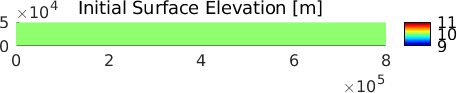
\includegraphics{/assets/img/tutorials/amr/amr_surface_initial.png}
	\end{center}
\end{figure}

\subsection{Transient solution with AMR}
In step 3, we specify which machine we want to run the model on, including number of processors to be used, define the model time step, final time, and prescribe the AMR frequency, i.e, how often the mesh needs to be updated. In this example, we run 500 yr forward in time to track the grounding line movement as soon as the initial thin ice slab starts to grounded on the bedrock. The ice starts to grounded in x=0, the boundary of the ice divide (vx=0 at x=0). We set the AMR frequency equal to 1, what means that the mesh is update (refined/coarsen) very time step). In this example, a time step equal to 1 yr is imposed. The SSA equations are used as the flow model.

Now that the set up is complete, we can run the model:
\begin{verbatim}md=solve(md,'Transient');\end{verbatim}

The solutions at the end of transient simulation (t=500 yr) can be visualized by plotting. Here, we plot the ice surface near the ice divide boundary (x=0 to x=250 km):
\begin{verbatim}finalstep=length(md.results.TransientSolution);
plotmodel(md,'data',md.results.TransientSolution(finalstep).Surface,'title','Surface Elevation
[m]','amr',finalstep,'xlim',[0 250000],'fontsize',12);\end{verbatim}
or in python:
\begin{verbatim}finalstep = len(md.results.TransientSolution) - 1
plotmodel(md, 'data', md.results.TransientSolution[-1].Surface, 'title', 'Surface Elevation [m]',
'amr', finalstep, 'xlim', [0, 250000], 'fontsize', 12, 'figure', 1)\end{verbatim}

\begin{figure}[H]
	\begin{center}
		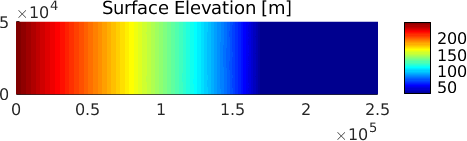
\includegraphics{/assets/img/tutorials/amr/amr_surface_final.png}
	\end{center}
\end{figure}

Here, we are plotting the mask grounded level set, which indicates if the ice is grounded (positive) or floating (negative). The value 0 indicates the position of the grounding line:
\begin{verbatim}finalstep=length(md.results.TransientSolution);
plotmodel(md,'data',md.results.TransientSolution(finalstep).MaskGroundediceLevelset,...
'title','Mask Grounded [m]','amr',finalstep,'xlim',[0 250000],'caxis',[-150 100],'fontsize',12);\end{verbatim}
or in python:
\begin{verbatim}plotmodel(md, 'data', md.results.TransientSolution[-1].MaskOceanLevelset,
'title', 'Mask Grounded [m]', 'amr', finalstep, 'xlim', [0, 250000], 'caxis', [-150, 100], 'fontsize', 12, 'figure', 2)\end{verbatim}

\begin{figure}[H]
	\begin{center}
		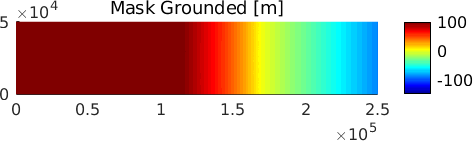
\includegraphics{/assets/img/tutorials/amr/amr_mask_final.png}
	\end{center}
\end{figure}

You can see the grounding line position is about x=170 km at the end of this example. To visualize the adaptive meshes, you can plot them at any saved time specifying the corresponding step:
\begin{verbatim}>> plotmodel(md,'data','mesh','amr',1,'xlim',[0 250000],'title','t=1 yr','fontsize',12,...
'data','mesh','amr',16,'xlim',[0 250000],'title','t=150 yr','fontsize',12,...
'data','mesh','amr',31,'xlim',[0 250000],'title','t=300 yr','fontsize',12,...
'data','mesh','amr',51,'xlim',[0 250000],'title','t=500 yr','fontsize',12);\end{verbatim}
or in python:
\begin{verbatim}plotmodel(md, 'data', 'mesh', 'amr', 0, 'xlim', [0, 250000], 'title', 't=1 yr', 'fontsize', 12,
'data', 'mesh', 'amr', 15, 'xlim', [0, 250000], 'title', 't=150 yr', 'fontsize', 12,
'data', 'mesh', 'amr', 30, 'xlim', [0, 250000], 'title', 't=300 yr', 'fontsize', 12,
'data', 'mesh', 'amr', 50, 'xlim', [0, 250000], 'title', 't=500 yr', 'fontsize', 12,
'figure', 3)\end{verbatim}

\begin{figure}[H]
	\begin{center}
		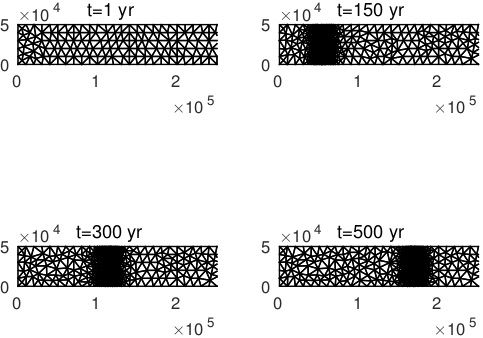
\includegraphics{/assets/img/tutorials/amr/amr_meshes.jpg}
	\end{center}
\end{figure}

To watch the evolution through time in an animation, we print the results and the respective meshes in .VTK-type file format, see the folder \verb@trunk/examples/AMR/@. These files can be seen using the ParaView (https://www.paraview.org/).

In ParaView, you will select which result to animate, and can watch the mesh tracking the grounding line movement as soon as the ice starts to grounded on the bedrock. The result and the mesh can be simultaneously displayed using selecting \verb@Surface With Edges@ in the box next to the field/result box selection.
